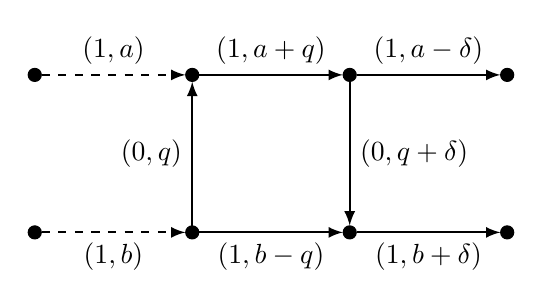
\begin{tikzpicture}[auto]

	\node (a1) [circle, scale=0.5, fill, draw] at (0, 2) {};
	\node (a2) [circle, scale=0.5, fill, draw] at (2, 2) {};
	\node (a3) [circle, scale=0.5, fill, draw] at (4, 2) {};
	\node (a4) [circle, scale=0.5, fill, draw] at (6, 2) {};
	\node (b1) [circle, scale=0.5, fill, draw] at (0, 0) {};
	\node (b2) [circle, scale=0.5, fill, draw] at (2, 0) {};
	\node (b3) [circle, scale=0.5, fill, draw] at (4, 0) {};
	\node (b4) [circle, scale=0.5, fill, draw] at (6, 0) {};

	\path[thick, -latex]
	(a1) edge[dashed] node {$(1,a)$} (a2)
	(a2) edge node {$(1,a+q)$} (a3)
	(a3) edge node {$(1,a-\delta)$} (a4)
	(b1) edge[dashed] node[below] {$(1,b)$} (b2)
	(b2) edge node[below] {$(1,b-q)$} (b3)
	(b3) edge node[below] {$(1,b+\delta)$} (b4)
	(b2) edge node[left] {$(0,q)$} (a2)
	(a3) edge node[right] {$(0,q+\delta)$} (b3);

\end{tikzpicture}
